\section{Results}
\label{sec:results}

In this section, ...


\subsection{Overall Overview}
\label{qual_res}


In our comprehensive exploration of 3D interfaces, the search term we employed was:
(gaming OR entertainment OR recreation OR games) AND ( VR OR virtual reality OR MR OR mixed reality) AND (wearables OR controller OR devices).

While our initial aim was to capture a holistic view of the entertainment and gaming industry, including its potential future trajectory, we also undertook a supplementary collection of health-related devices. We decided on this as even though our search term was not intended to find papers concerning health-related devices, the IEEExplore Library still provided papers in that direction. This was considered as reasonable as it would also allow as to of forecasting the evolution of 3D interfaces from the healthcare sector into the entertainment sector.

However, we did not evaluate the health-related devices in detail only included them in our broad categorization, seen in Figure..,. A few reasons underscored this decision:

Health-related devices are designed for specialized tasks. Their functionalities and implications are vast, often requiring a detailed, domain-specific understanding which differed from our primary sectors of focus.

While one of our sub goals was to forecast future trends, the sheer breadth and depth of the health domain hinted at a vast potential that would be best addressed in a dedicated study.

Given these considerations, we believed it was in the best interest of the study's clarity and precision to focus on the domains outlined by our original search terms: Gaming, Entertainment, and Recreation. 


\begin{figure}[htbp]
	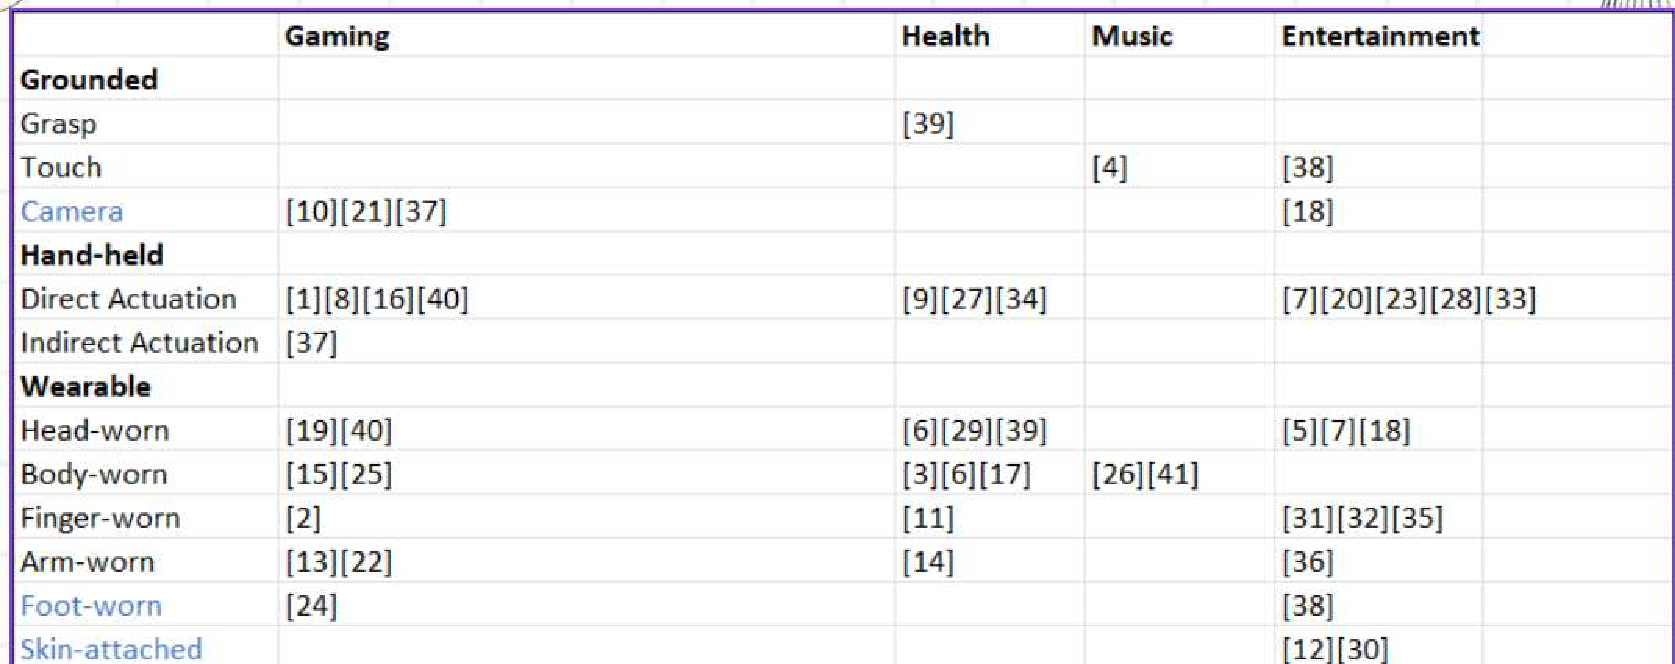
\includegraphics[width=\columnwidth]{figures/broad.pdf}
	\label{fig:broad}
\end{figure}

\subsection{Gaming}
\label{gaming}


In the explanation and chart for the gaming landscape we have looked at 3D interfaces, especially as they address to virtual and mixed reality. Through a detailed bottom-up approach we have categorized these interfaces based which body part used the device. 
Starting with the Grounded devices, think of these as the dependable tools that stay put. Which is subcategorized for Visual and Contact. “Visual" tools rely on our sense of sight, while "Contact" ones require a hands-on approach. Then the primarily include visual gadgets like cameras and infrared sensors. 

\begin{figure}[htbp]
	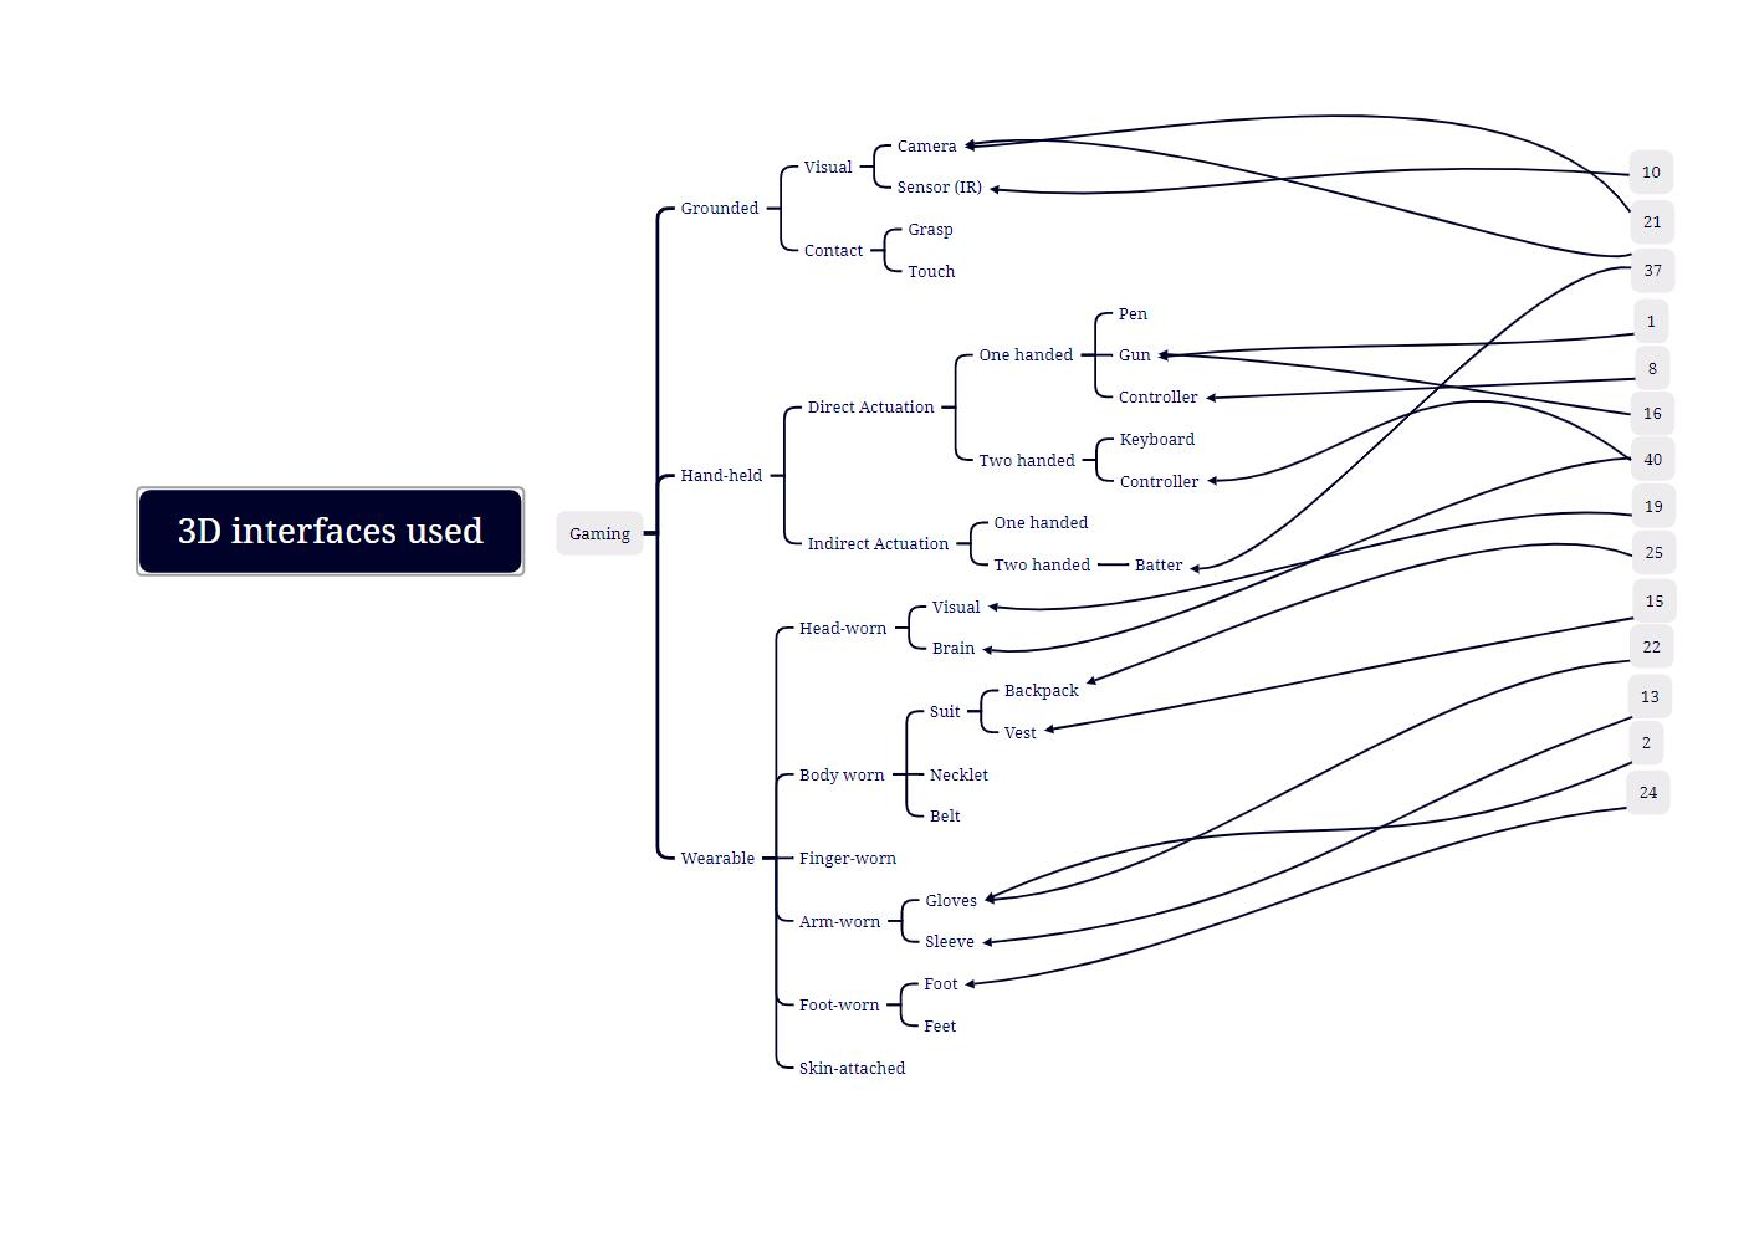
\includegraphics[width=\columnwidth]{figures/gaming.pdf}
	\label{fig:gaming}
\end{figure}

Then there is also the tactile world of Contact Interfaces, which involve direct touch or grasping actions. 

Then there's the Hand-held category, the tools you can pick up and play with for example like the pens and guns. Wearable interfaces are the ones that you wear on your head, your body, or even attached to your skin. From the high-tech brain interface devices to the more common wearables for specific body parts.

\subsection{Entertainment}
\label{entertainment}

\begin{figure}[htbp]
	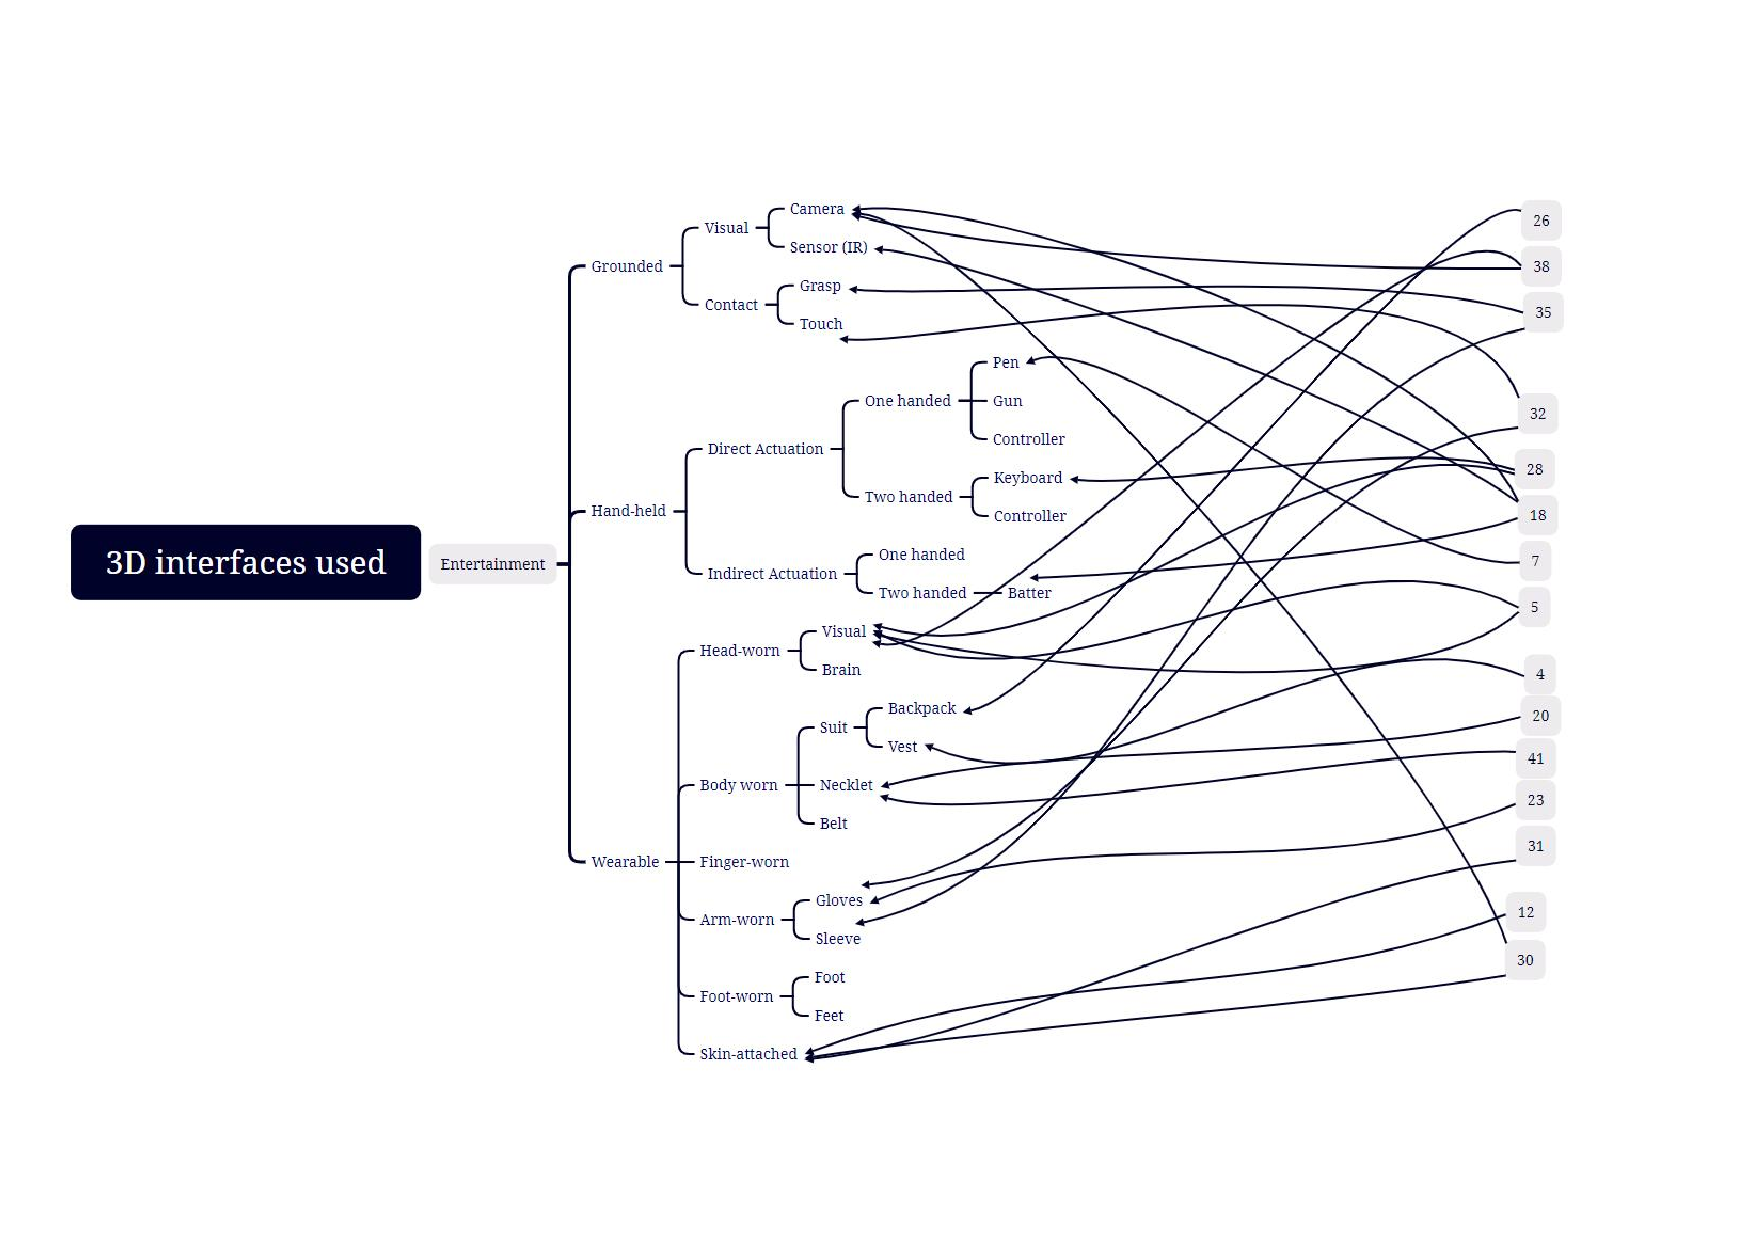
\includegraphics[width=\columnwidth]{figures/entertainment.pdf}
	\label{fig:entertainment}
\end{figure}


\subsection{Outstanding Devices}
VR treadmill system (leap motion) coupled with a handheld 3D interface. The device is meant to be used for whole body and detect a leap when necessary. Gaming has added a new perspective on jumping over objects and it's a key movement on games these days. The sensors work simultaneously so the axis also can be changed with a little offset as well.

Haptic sensors for feet, can be used to define the motion of and placement. The sensors are meant to be used with two feet at the time but they also can be used individually for different kind of tasks. 

A high-fidelity and high-precision multi-surface pen for virtual reality. With the pen the drawing does not only happen in a 2D space like we have been used to, it can also create objects and multiple different lines in 3D space making the visual outcome a lot of different compared to the normal pen that we are used to.

Soft microtubule muscle-driven 3-axis skin-stretch haptic device. The device tracks basically movement on a very high accuracy, so completing tasks with fingers like some different grips are made to be more normal and the feedback feels more like real life.

The design and implementation of a VR gun controller with haptic feedback. The gun(s) have a feedback motor and when attached to a real print of the gun added to visual devices will give the user experience like being in a real situation. Without the feedback it would feel more poor and have a lack of sensation. The motor it's self is quite simple creation but the way they have included it in a bigger entity makes it create a whole new level to the gaming.

Wack-a-mole styled hammer for games. The tool itself has a sensors, but it's also being tracked by cameras that have been grounded next to the system. The user can either see the gameplay happening on screen or by using a visual headset (VR). The second will create a more live-like experience due the high precision for it.

\subsection{something something}

The importance of subcategories becomes evident when examining user interactions. While broad categories provide an overview of interface options, the subcategories offer tailored solutions that cater to individual needs. For example, within the realm of hand-held interfaces, choices extend beyond general preferences. Some users may favor a one-handed controller due to its ergonomic design, which can minimize arm strain and align better with natural postures. Others might gravitate towards a two-handed controller, valuing its stability and comprehensive button layout. By diving into these specific nuances, we can design interfaces that not only meet functional requirements but also prioritize user comfort and intuitive use. This meticulous attention to detail ensures enhanced usability and heightened user satisfaction.